\documentclass[letterpaper, 10 pt, conference]{ieeeconf}

\IEEEoverridecommandlockouts
\overrideIEEEmargins

\usepackage[utf8]{inputenc}
\usepackage[T1]{fontenc}
\usepackage{amsmath}
\usepackage{amssymb}
\usepackage{booktabs}
\usepackage{graphicx}
\usepackage{multirow}
\usepackage{xcolor}
\usepackage{url}

\newcommand{\method}{ForeTac}
\newcommand{\Real}{\mathbb{R}}
\newcommand{\loss}{\mathcal{L}}
\newcommand{\marker}{\mathbf{m}}
\newcommand{\action}{\mathbf{a}}
\newcommand{\obs}{\mathbf{o}}
\newcommand{\latent}{\mathbf{z}}
\newcommand{\score}{S}
\newcommand{\tbd}{TBD}

\graphicspath{{figures/}{./}}

\title{\LARGE \bf
Supplementary Material for \method{}: Steering Robot Actions with Predicted Contact Consequences}

\author{Anonymous Authors}

\begin{document}

\maketitle
\thispagestyle{empty}
\pagestyle{empty}
\raggedbottom

\section{Appendix Overview}

This appendix provides implementation details and additional evidence for
\method{}. Section~\ref{sec:data} describes the real-robot data format and the
current local data inventory. Section~\ref{sec:training} gives training and
deployment hyperparameters. Section~\ref{sec:algorithm} expands the algorithmic
pipeline. Sections~\ref{sec:encoder}--\ref{sec:guidance} report the tactile
encoder, foresight, scorer, force-curve, main-comparison, and ablation results.
Some controlled online rollouts and qualitative image panels are still being
collected; entries that are not yet verified are left as \tbd{}.

\section{Data Collection and Format}
\label{sec:data}

\subsection{Robot Observation Schema}

All policies and foresight modules are trained from timestamp-aligned HDF5
episodes. A trajectory contains synchronized RGB views, proprioception, action
labels, tactile marker fields, and optional force/torque measurements. The main
action-conditioned foresight contract is
\begin{equation}
\hat{\latent}_{t:t+H-1}
= f_\psi(I_t^g, I_t^w, \marker_{t-W+1:t}, q_t,
\action_{t:t+H-1}),
\end{equation}
where the condition is the future action chunk
\texttt{actions/joint\_abs[t:t+H]}, not the future state trajectory. This
distinction is important: future states are outcomes, while the rollout-time
quantity available before execution is the candidate action chunk.

\begin{table}[t]
\caption{HDF5 episode fields used by the current implementation.}
\label{tab:hdf5_schema}
\centering
\resizebox{\columnwidth}{!}{%
\begin{tabular}{lll}
\toprule
Field & Shape / type & Usage\\
\midrule
\texttt{observations/images/global} & $T \times H \times W \times 3$ uint8 & scene context\\
\texttt{observations/images/wrist} & $T \times H \times W \times 3$ uint8 & local contact geometry\\
\texttt{observations/proprio\_joint} & $T \times 7$ float & current robot state\\
\texttt{actions/joint\_abs} & $T \times 7$ float & action chunk target / foresight condition\\
\texttt{observations/tac/left/marker\_offset} & $T \times 9 \times 9 \times 2$ float & GelSight marker displacement\\
\texttt{observations/tac/left/force6d} & $T \times 6$ float & contact-quality labels and analysis\\
\bottomrule
\end{tabular}%
}
\end{table}

RGB images are resized and cropped before ImageNet normalization. The tactile
input is a GelSight marker displacement field, normalized per displacement
channel. TacVAE consumes an eight-frame tactile window and encodes the current
contact into a compact spatial latent. The diffusion policy uses
\texttt{obs\_horizon}=2 and predicts a 16-step action chunk for the main
experiments.

\subsection{Current Local Data Inventory}

Table~\ref{tab:data_inventory} lists the data currently visible in the local
workspace and used by the corresponding training/evaluation scripts. The board
split is the labeled board TacVAE split; card and vase splits are the current
task-specific TacVAE splits; insertion uses the truncated insertion datasets
for policy and score-model development.

\begin{table*}[t]
\caption{Current local episode inventory. Counts are from the local HDF5
directories and saved split metrics.}
\label{tab:data_inventory}
\centering
\setlength{\tabcolsep}{4pt}
\resizebox{\textwidth}{!}{%
\begin{tabular}{llcl}
\toprule
Task & Main local sources & Episodes / split & Primary role\\
\midrule
Board wiping &
\texttt{260609/wipe\_pos}, \texttt{z\_too\_high}, \texttt{260610/z\_too\_low}, \texttt{z\_too\_oscillate} &
177 train / 44 test; 9631 test windows &
TacVAE, force-band scorer, action-conditioned foresight\\
Board wiping extra positives &
\texttt{260617\_v8l\_caheiban/peg\_in\_hole\_0617} &
80 episodes &
positive contact reference and rollout validation\\
Vase wiping &
\texttt{260630\_v8j\_huaping/peg\_in\_hole\_0630} &
90 train / 10 test; 2088 test windows &
TacVAE and contact-stability analysis\\
Card swiping &
\texttt{260615\_v8l\_card}, \texttt{260626\_replay\_card}, \texttt{260629/260701\_v8j\_card} &
246 train / 27 test; 6033 test windows &
TacVAE and card positive/negative data analysis\\
Chip grasping &
\tbd{} &
\tbd{} &
fragile grasp rollout table placeholder\\
Socket insertion &
\texttt{0209-0210\_truncated}, \texttt{260401\_k14\_truncated} &
318 + 162 episodes visible locally &
insertion policy/scorer development and 20-trial benchmark\\
\bottomrule
\end{tabular}%
}
\end{table*}

\subsection{Task Labels and Safety Definitions}

For each online trial, a success is counted when the task objective is completed
within the rollout horizon. A safe success is stricter: the task must succeed
without contact-force violations, object disturbance, emergency stops, or
task-specific unsafe modes. The task-specific safety rules are:
\begin{itemize}
\item Board wiping: stable moderate force over the wipe path, with no long
contact dropout and no force spike above the allowed band.
\item Vase wiping: continuous contact on the curved surface, low object motion,
and no tip-over or high-force spike.
\item Card swiping: sustained slot contact and successful pass-through without
dropout or large misalignment.
\item Chip grasping: lift without crushing or slipping.
\item Socket insertion: insertion success with bounded peak force, limited
retry count, and no sustained jamming.
\end{itemize}

\section{Training Details}
\label{sec:training}

\subsection{Model Components}

Table~\ref{tab:train_hparams} summarizes the implementation settings used in
the current experiments. These values match the local scripts and configs used
for the project page and appendix evidence.

\begin{table*}[t]
\caption{Main training hyperparameters.}
\label{tab:train_hparams}
\centering
\setlength{\tabcolsep}{4pt}
\resizebox{\textwidth}{!}{%
\begin{tabular}{llll}
\toprule
Component & Architecture / input & Optimization & Notes\\
\midrule
TacVAE &
8-frame $9 \times 9 \times 2$ marker windows; latent $16 \times 3 \times 3$ &
AdamW, lr $10^{-4}$, batch 512, 150 epochs, stride 2 or 4 &
KL weight $10^{-6}$; direction loss weight 0.2\\
Visual/tactile DP &
global+wrist RGB, TacVAE latent history, $q_t$; action horizon 16 &
AdamW, lr $10^{-4}$, batch 64, 1000 epochs for board &
DDPM training steps 100; inference steps 100; action space \texttt{joint\_abs}\\
Action-conditioned foresight &
ResNet18 visual tokens, TacVAE tokens, $q_t$, action chunk $H=16$ &
AdamW, lr $4{\times}10^{-5}$, weight decay $10^{-4}$ &
3 transformer layers, 8 heads, hidden 512, FFN 2048\\
Contact-quality scorer &
predicted latent sequence and optional action/force features &
cross-entropy / margin objective &
deployed score is expert-good margin against negative modes\\
Guided denoising &
late DDPM steps only &
normalized gradient step; trust-region clipping &
action branch detached in latent-only path\\
\bottomrule
\end{tabular}%
}
\end{table*}

\subsection{Foresight Loss}

The foresight model predicts the latent sequence corresponding to the candidate
action chunk. Training uses frozen TacVAE targets and combines three terms:
\begin{align}
\loss_{\rm fs}
&= \loss_{\rm latent}
+ \lambda_m \loss_{\rm marker}
+ \lambda_\Delta \loss_\Delta,\\
\loss_{\rm latent}
&= {\rm SmoothL1}(\hat{\latent}_{1:H}, \latent_{1:H})
+ {\rm SmoothL1}(\hat{\latent}_H, \latent_H),\\
\loss_{\rm marker}
&= {\rm SmoothL1}(D_{\rm tac}(\hat{\latent}_{1:H}), \marker_{1:H}),\\
\loss_\Delta
&= {\rm SmoothL1}(\Delta\hat{\latent}_{1:H-1},
\Delta\latent_{1:H-1}).
\end{align}
The main configuration uses $\lambda_m=0.3$ and $\lambda_\Delta=0.5$. Decoded
marker loss keeps the latent forecast physically tied to marker displacement,
while the delta term penalizes temporally inconsistent predictions.

\subsection{Correct Action Conditioning}

The current corrected training path sets \texttt{use\_state\_trajectory=false}.
For a sample starting at time $t$, the foresight input is
\texttt{actions/joint\_abs[t:t+H]} and the target is the tactile future
\texttt{marker\_offset[t+1:t+H]} or the stride-aligned equivalent. The previous
state-trajectory mode is kept only as a legacy option for ablations and should
not be used for the main \method{} claim.

\section{Algorithmic Pipeline}
\label{sec:algorithm}

\noindent\textbf{Algorithm S1: Inference-time predicted-contact guidance.}
\begin{enumerate}
\item Read the current observation $\obs_t=(I_t^g,I_t^w,q_t,
\marker_{t-W+1:t})$.
\item Encode the tactile history with TacVAE to obtain the current latent
$\latent_t$ and tactile tokens.
\item Run the base action generator to sample a denoising trajectory for an
action chunk $\action_{t:t+H-1}$.
\item At selected late denoising steps, convert the noisy action sample to the
clean action estimate $\hat{x}_0$.
\item Feed $\hat{x}_0$ into the action-conditioned foresight model and predict
the future tactile latent sequence
$\hat{\latent}_{t:t+H_f-1}$.
\item Score the predicted tactile future with the contact-quality energy model:
\begin{equation}
s_{\rm margin}
= \ell_{\rm good}
- \log \sum_{c \in \mathcal{C}_{\rm bad}} \exp(\ell_c).
\end{equation}
\item Backpropagate $s_{\rm margin}$ through
$\action \rightarrow \hat{\latent} \rightarrow \score$ and apply a normalized
small update inside a raw-action trust region.
\item Execute only the first action steps of the refined chunk and repeat at
the next control cycle.
\end{enumerate}

This design separates behavior generation from contact-quality correction. The
base policy remains the prior over demonstrated robot motions; foresight asks
what tactile consequence a candidate chunk would create; the scorer decides
whether that predicted future contact is desirable.

\section{Tactile Encoder and Reconstruction}
\label{sec:encoder}

\subsection{Encoder Construction}

TacVAE uses an encoder-decoder structure over marker displacement fields rather
than raw tactile images. The input is an eight-frame marker window; the encoder
maps it to a $16 \times 3 \times 3$ spatial latent and the decoder reconstructs
a $9 \times 9 \times 2$ marker field. The spatial latent keeps local contact
geometry available to foresight and the scorer, while reducing the regression
target from raw marker grids to a compact contact representation.

\begin{table*}[t]
\caption{Reconstruction comparison across tactile encoders. Each task reports
MAE / cosine similarity. Best available values in each task-metric column are
bolded.}
\label{tab:encoder_recon}
\centering
\setlength{\tabcolsep}{4pt}
\resizebox{\textwidth}{!}{%
\begin{tabular}{lcccccccc}
\toprule
\multirow{2}{*}{Encoder} &
\multicolumn{2}{c}{Board} &
\multicolumn{2}{c}{Vase} &
\multicolumn{2}{c}{Card} &
\multicolumn{2}{c}{Chip}\\
\cmidrule(lr){2-3}\cmidrule(lr){4-5}\cmidrule(lr){6-7}\cmidrule(lr){8-9}
& MAE $\downarrow$ & Cos. $\uparrow$
& MAE $\downarrow$ & Cos. $\uparrow$
& MAE $\downarrow$ & Cos. $\uparrow$
& MAE $\downarrow$ & Cos. $\uparrow$\\
\midrule
PCA & 0.040 & 0.995 & 0.035 & \textbf{0.995} & 0.036 & 0.980 & 0.026 & 0.965\\
PointNet-AE & 0.048 & 0.956 & \textbf{0.027} & 0.955 & 0.044 & 0.992 & 0.032 & \textbf{0.990}\\
Conv-AE & 0.055 & 0.997 & 0.042 & 0.994 & 0.104 & \textbf{0.999} & 0.036 & 0.959\\
TacVAE (ours) & \textbf{0.039} & \textbf{0.998} & 0.037 & 0.975 & \textbf{0.031} & \textbf{0.999} & \textbf{0.015} & 0.899\\
\bottomrule
\end{tabular}%
}
\end{table*}

\subsection{Interpretation}

The reconstruction table shows that the marker field is low-dimensional enough
for simple baselines to reconstruct many static frames. This is why
reconstruction alone is not the full argument for TacVAE. The relevant property
for \method{} is whether the latent is useful in the full differentiable chain:
current tactile history $\rightarrow$ future tactile prediction
$\rightarrow$ contact-quality score $\rightarrow$ action update. TacVAE is
therefore evaluated together with foresight prediction and guidance
diagnostics, not only as a standalone autoencoder.

\section{Foresight Prediction Quality}
\label{sec:foresight}

The horizon study evaluates whether a longer predicted tactile future improves
action selection despite the expected degradation in prediction error.
Table~\ref{tab:foresight_horizon} reports the current board-wiping numbers.
The 16-step horizon is the main setting and matches the main online success
rate used by the controller. Short horizons have lower reconstruction error but
do not expose enough future contact consequence for stable guidance.

\begin{table}[t]
\caption{Foresight prediction quality and rollout success across prediction
horizons.}
\label{tab:foresight_horizon}
\centering
\resizebox{\columnwidth}{!}{%
\begin{tabular}{ccccc}
\toprule
Horizon & Latent MAE $\downarrow$ & Latent cosine $\uparrow$ & Marker error $\downarrow$ & Success $\uparrow$\\
\midrule
1 & 0.167 & 0.9993 & 0.213 px & 60\%\\
4 & 0.188 & 0.9989 & 0.297 px & 68\%\\
8 & 0.230 & 0.9965 & 0.317 px & 75\%\\
12 & 0.261 & 0.9952 & 0.352 px & 80\%\\
16 & 0.274 & 0.9953 & 0.377 px & \textbf{85\%}\\
\bottomrule
\end{tabular}%
}
\end{table}

\begin{figure}[t]
  \centering
  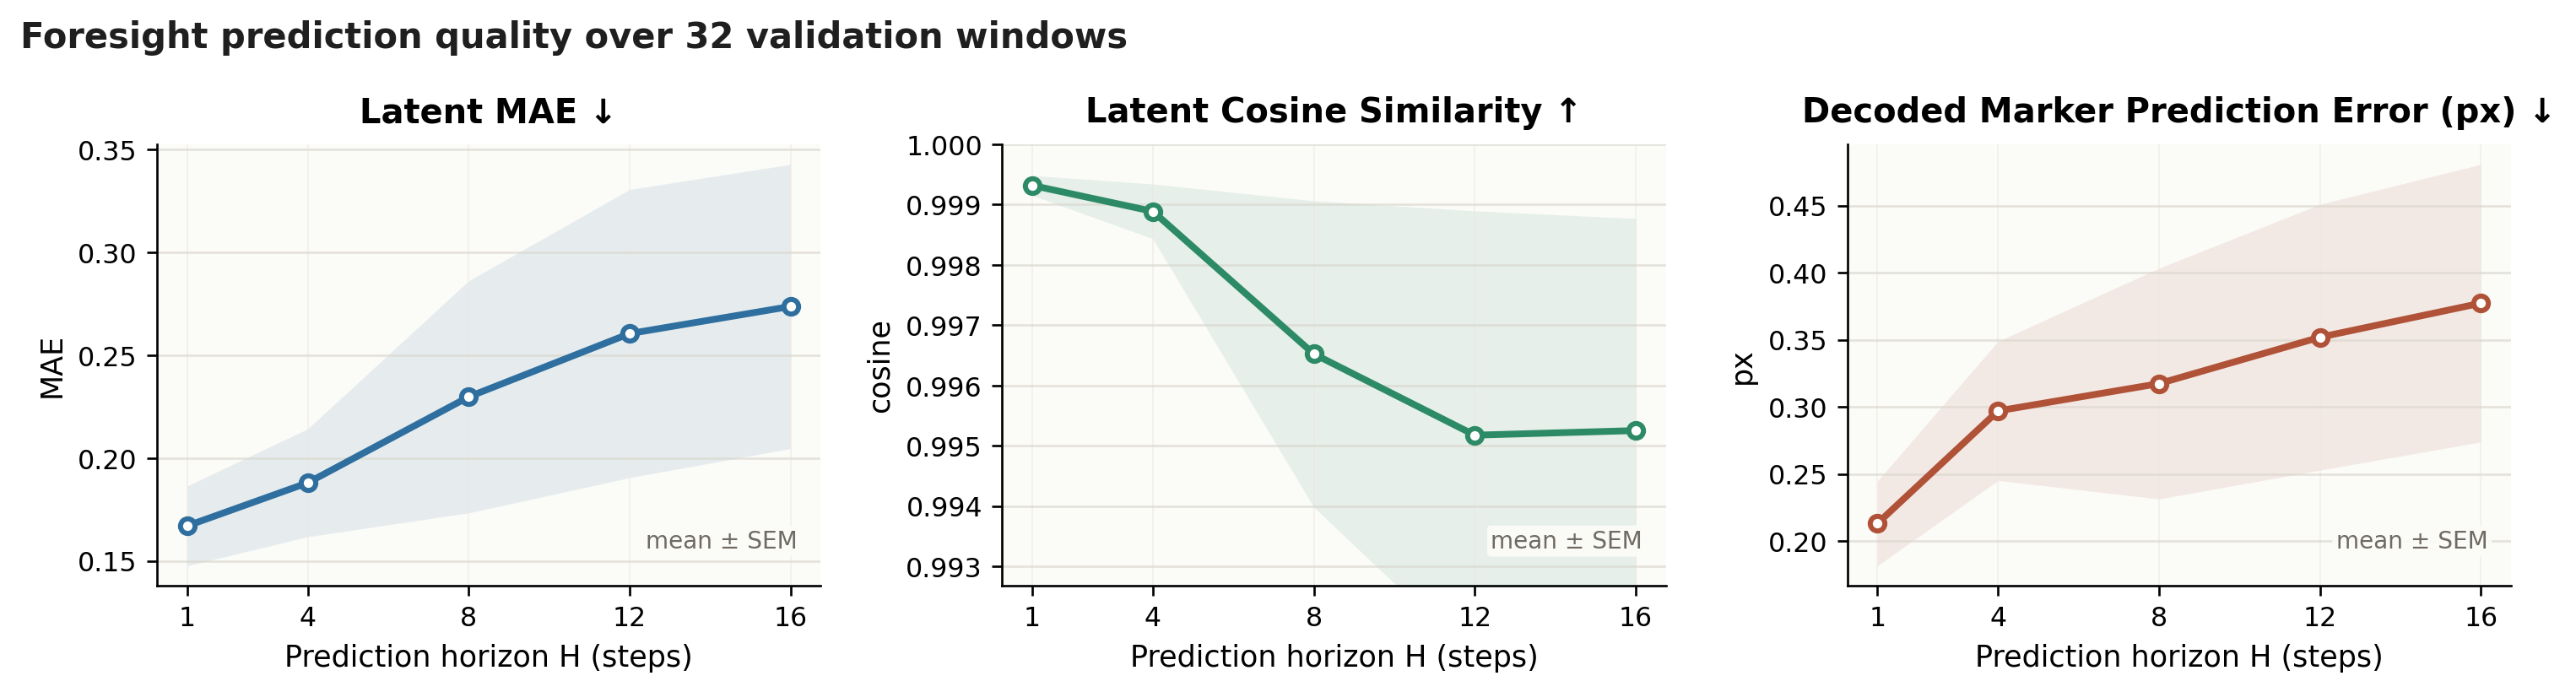
\includegraphics[width=0.98\linewidth]{figures/foresight_prediction_quality_horizons.png}
  \caption{Foresight prediction quality across horizons. Longer horizons have
  larger decoded marker error, but provide more task-relevant future contact
  context for action guidance.}
  \label{fig:appendix_foresight_curve}
\end{figure}

\begin{figure}[t]
  \centering
  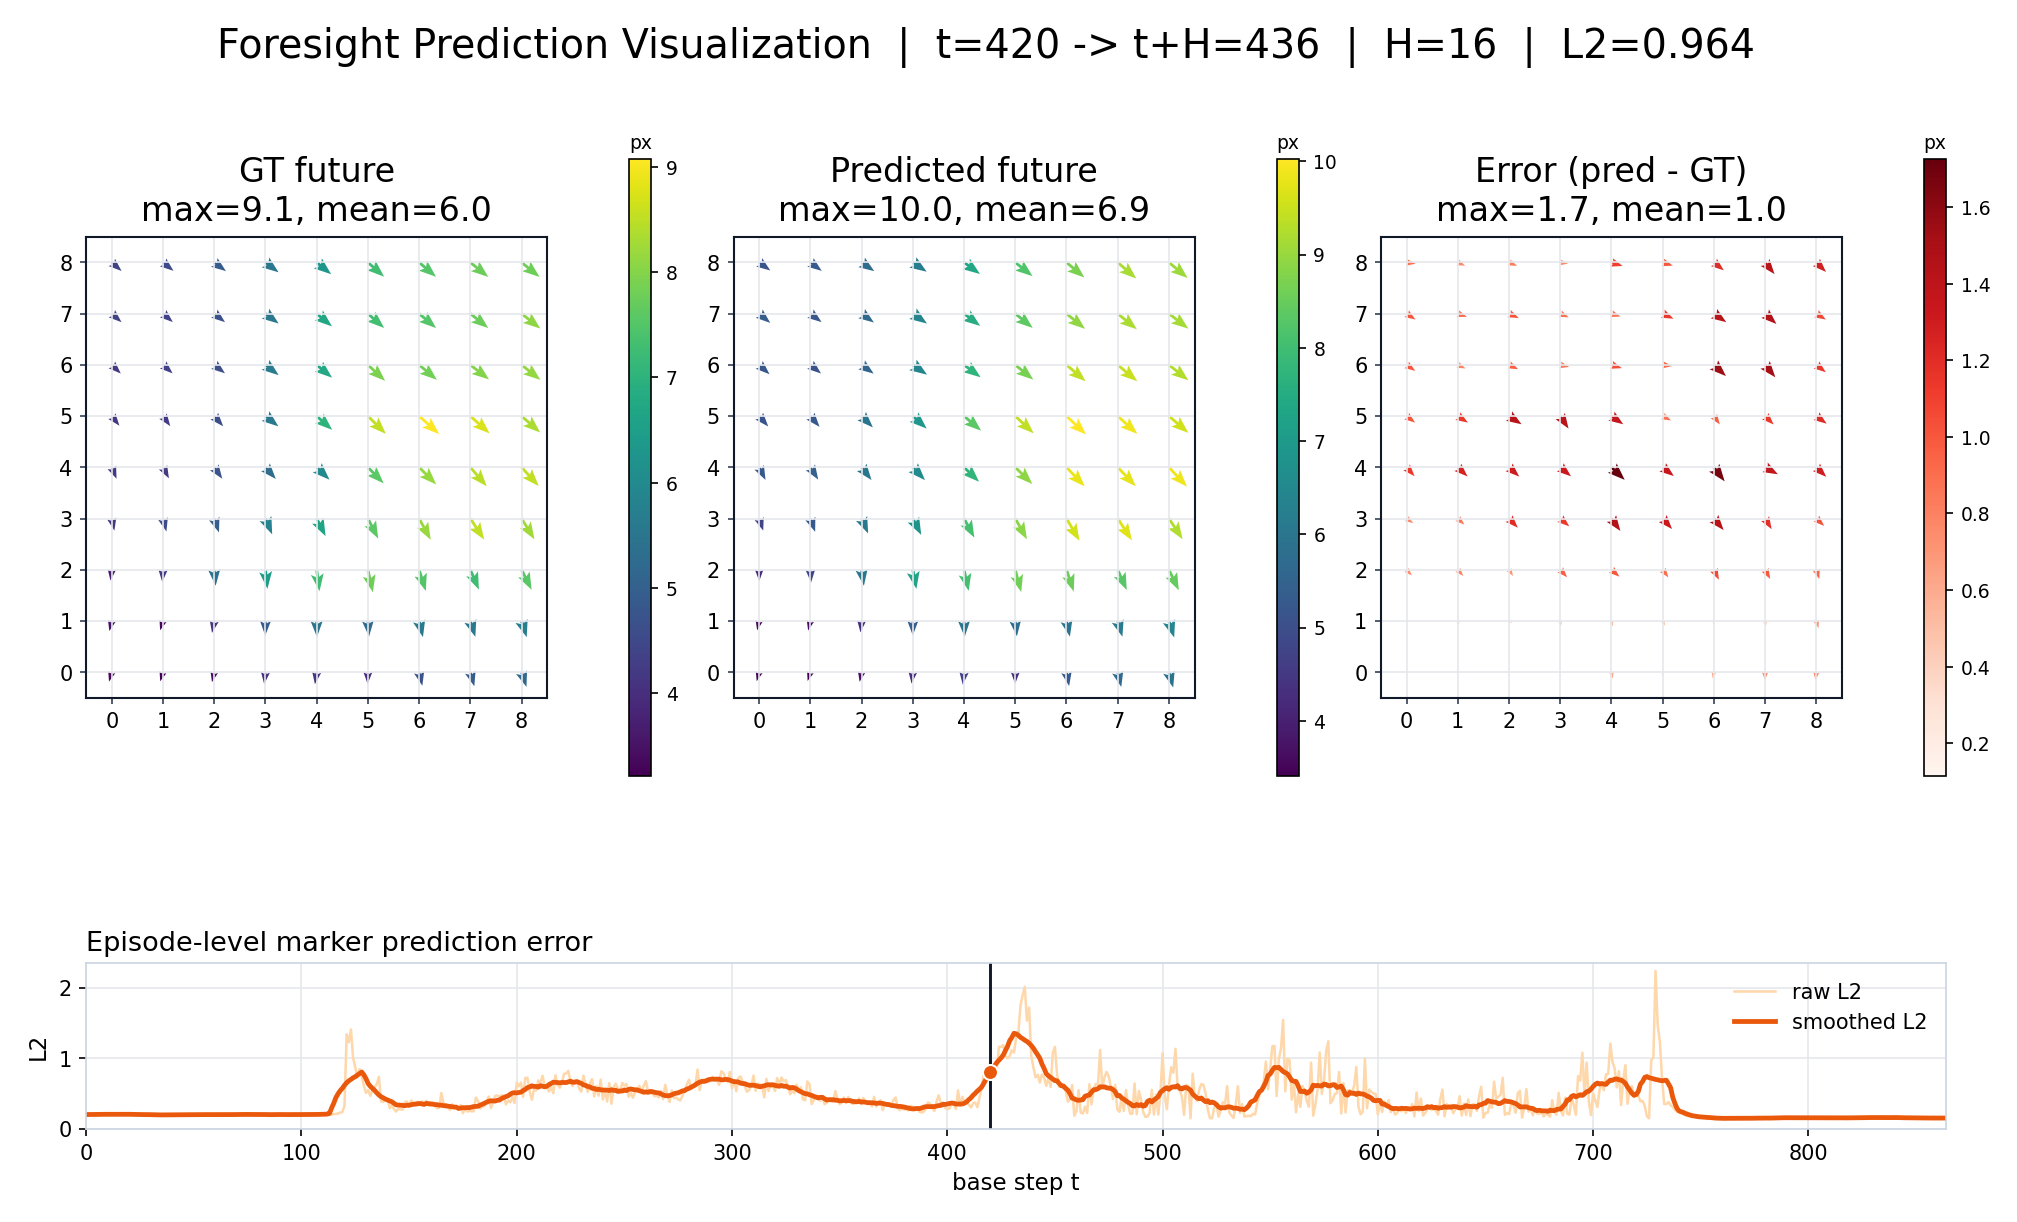
\includegraphics[width=0.98\linewidth]{figures/foresight_prediction_board_episode6_tplus16_summary.png}
  \caption{Example long-horizon board prediction. The predicted marker field
  preserves the contact direction and spatial contact pattern needed by the
  scorer.}
  \label{fig:appendix_foresight_example}
\end{figure}

\section{Contact-Quality Scorer Validation}
\label{sec:scorer}

\subsection{Preference-Order Accuracy}

The scorer is validated with positive/negative rollout pairs. For each pair, a
key contact frame is selected from the offline rollout. The pair is counted as
correct when the positive rollout receives a higher score than the negative
rollout. This validates the ranking property required by the energy model: the
absolute score does not need to be calibrated perfectly, but the positive
contact segment should score above the failure segment.

\begin{table*}[t]
\caption{Offline preference-order validation on the current board smoke rollout
subset.}
\label{tab:preference_order}
\centering
\setlength{\tabcolsep}{6pt}
\resizebox{\textwidth}{!}{%
\begin{tabular}{lccccc}
\toprule
Selection rule & Score type & Correct / pairs & Accuracy & Mean gap & Median gap\\
\midrule
Key marker frame & expert margin & 2 / 3 & 0.6667 & 0.033707 & 0.024794\\
Key marker frame & quality 0--100 & 2 / 3 & 0.6667 & 0.000956 & 0.000685\\
Key force frame & expert margin & 2 / 3 & 0.6667 & -0.012368 & 0.016713\\
Model-best window & expert margin & 2 / 3 & 0.6667 & 0.060702 & 0.092206\\
Model-best window & quality 0--100 & 2 / 3 & 0.6667 & 0.001863 & 0.002820\\
All windows & expert margin & 1090 / 2436 & 0.4475 & -0.003016 & -0.006750\\
All windows & quality 0--100 & 1090 / 2436 & 0.4475 & -0.000048 & -0.000190\\
\bottomrule
\end{tabular}%
}
\end{table*}

The key-frame and model-best selections are more meaningful than averaging all
windows because most non-contact or low-contact windows are ambiguous and do
not reflect the decisive contact event. The current smoke subset is small, so
the table is evidence for scorer behavior rather than a formal final result.
The next complete validation should use all rollout pairs collected under the
same initial-condition protocol.

\subsection{Gradient and Sampler Diagnostics}

The scorer must also be usable as a differentiable guidance signal. The board
stride-3 diagnostic verifies that the composed
action--foresight--score chain produces finite gradients and bounded action
updates.

\begin{table}[t]
\caption{Board stride-3 guidance diagnostic.}
\label{tab:guidance_diag_appendix}
\centering
\begin{tabular}{lc}
\toprule
Metric & Value\\
\midrule
Validation windows & 3144\\
Scorer accuracy / macro-F1 & 1.000 / 1.000\\
Expert-margin AUROC & 1.000\\
Rows with finite gradients & 128 / 128\\
Mean raw gradient norm & 2.4475\\
Mean scaled gradient norm & 0.00734\\
Mean guided-step score delta & 0.0198\\
Mean applied update norm & 0.0030\\
\bottomrule
\end{tabular}
\end{table}

\begin{figure*}[t]
  \centering
  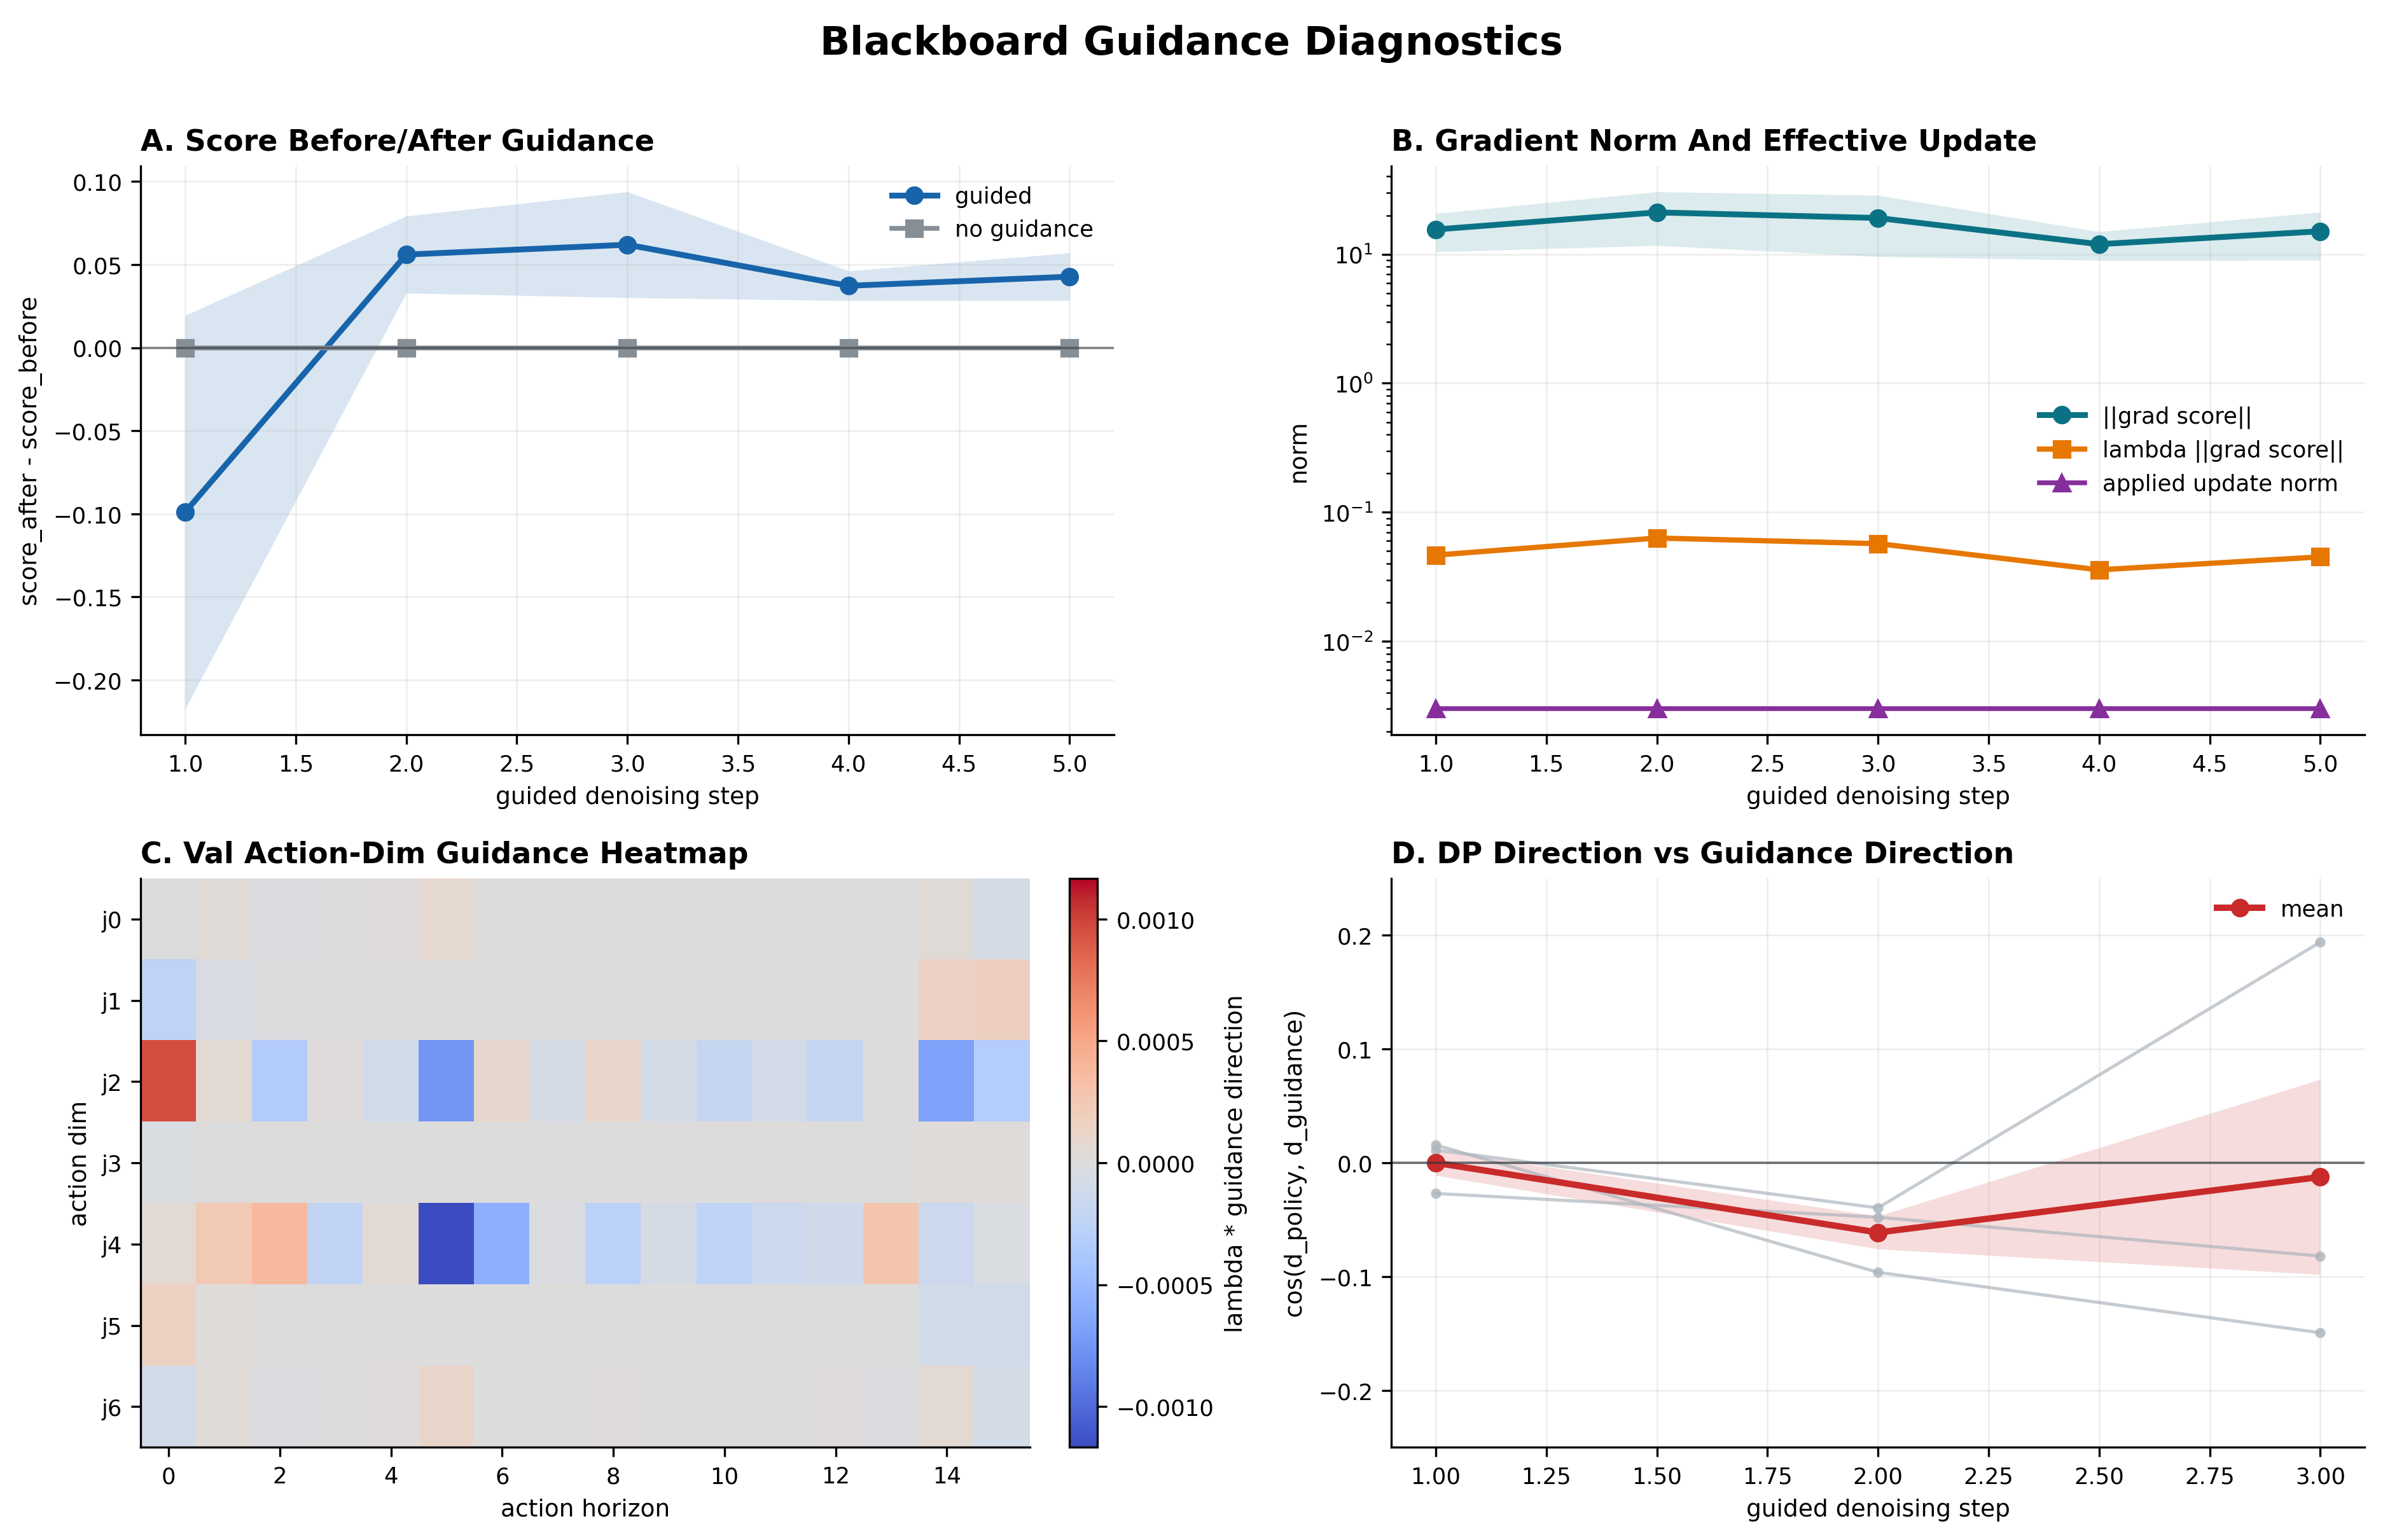
\includegraphics[width=0.92\textwidth]{figures/board_guidance_diagnostics_overview.png}
  \caption{Board guidance visualizations. The panels summarize score changes,
  gradient magnitude, action-dimension localization, and policy-guidance
  alignment. The update is finite and localized, consistent with a small
  contact correction rather than a full trajectory rewrite.}
  \label{fig:appendix_guidance_overview}
\end{figure*}

\section{Force-Curve Analysis}
\label{sec:force}

Force traces provide an interpretable view of the contact-quality objective.
For wiping tasks, the desired behavior is not maximum force. The desired
behavior is a stable force band that maintains contact without disturbing the
object. For insertion, the desired behavior is bounded peak force plus few
retries; a policy that keeps pushing after contact can look geometrically
reasonable but is unsafe.

\begin{figure*}[t]
  \centering
  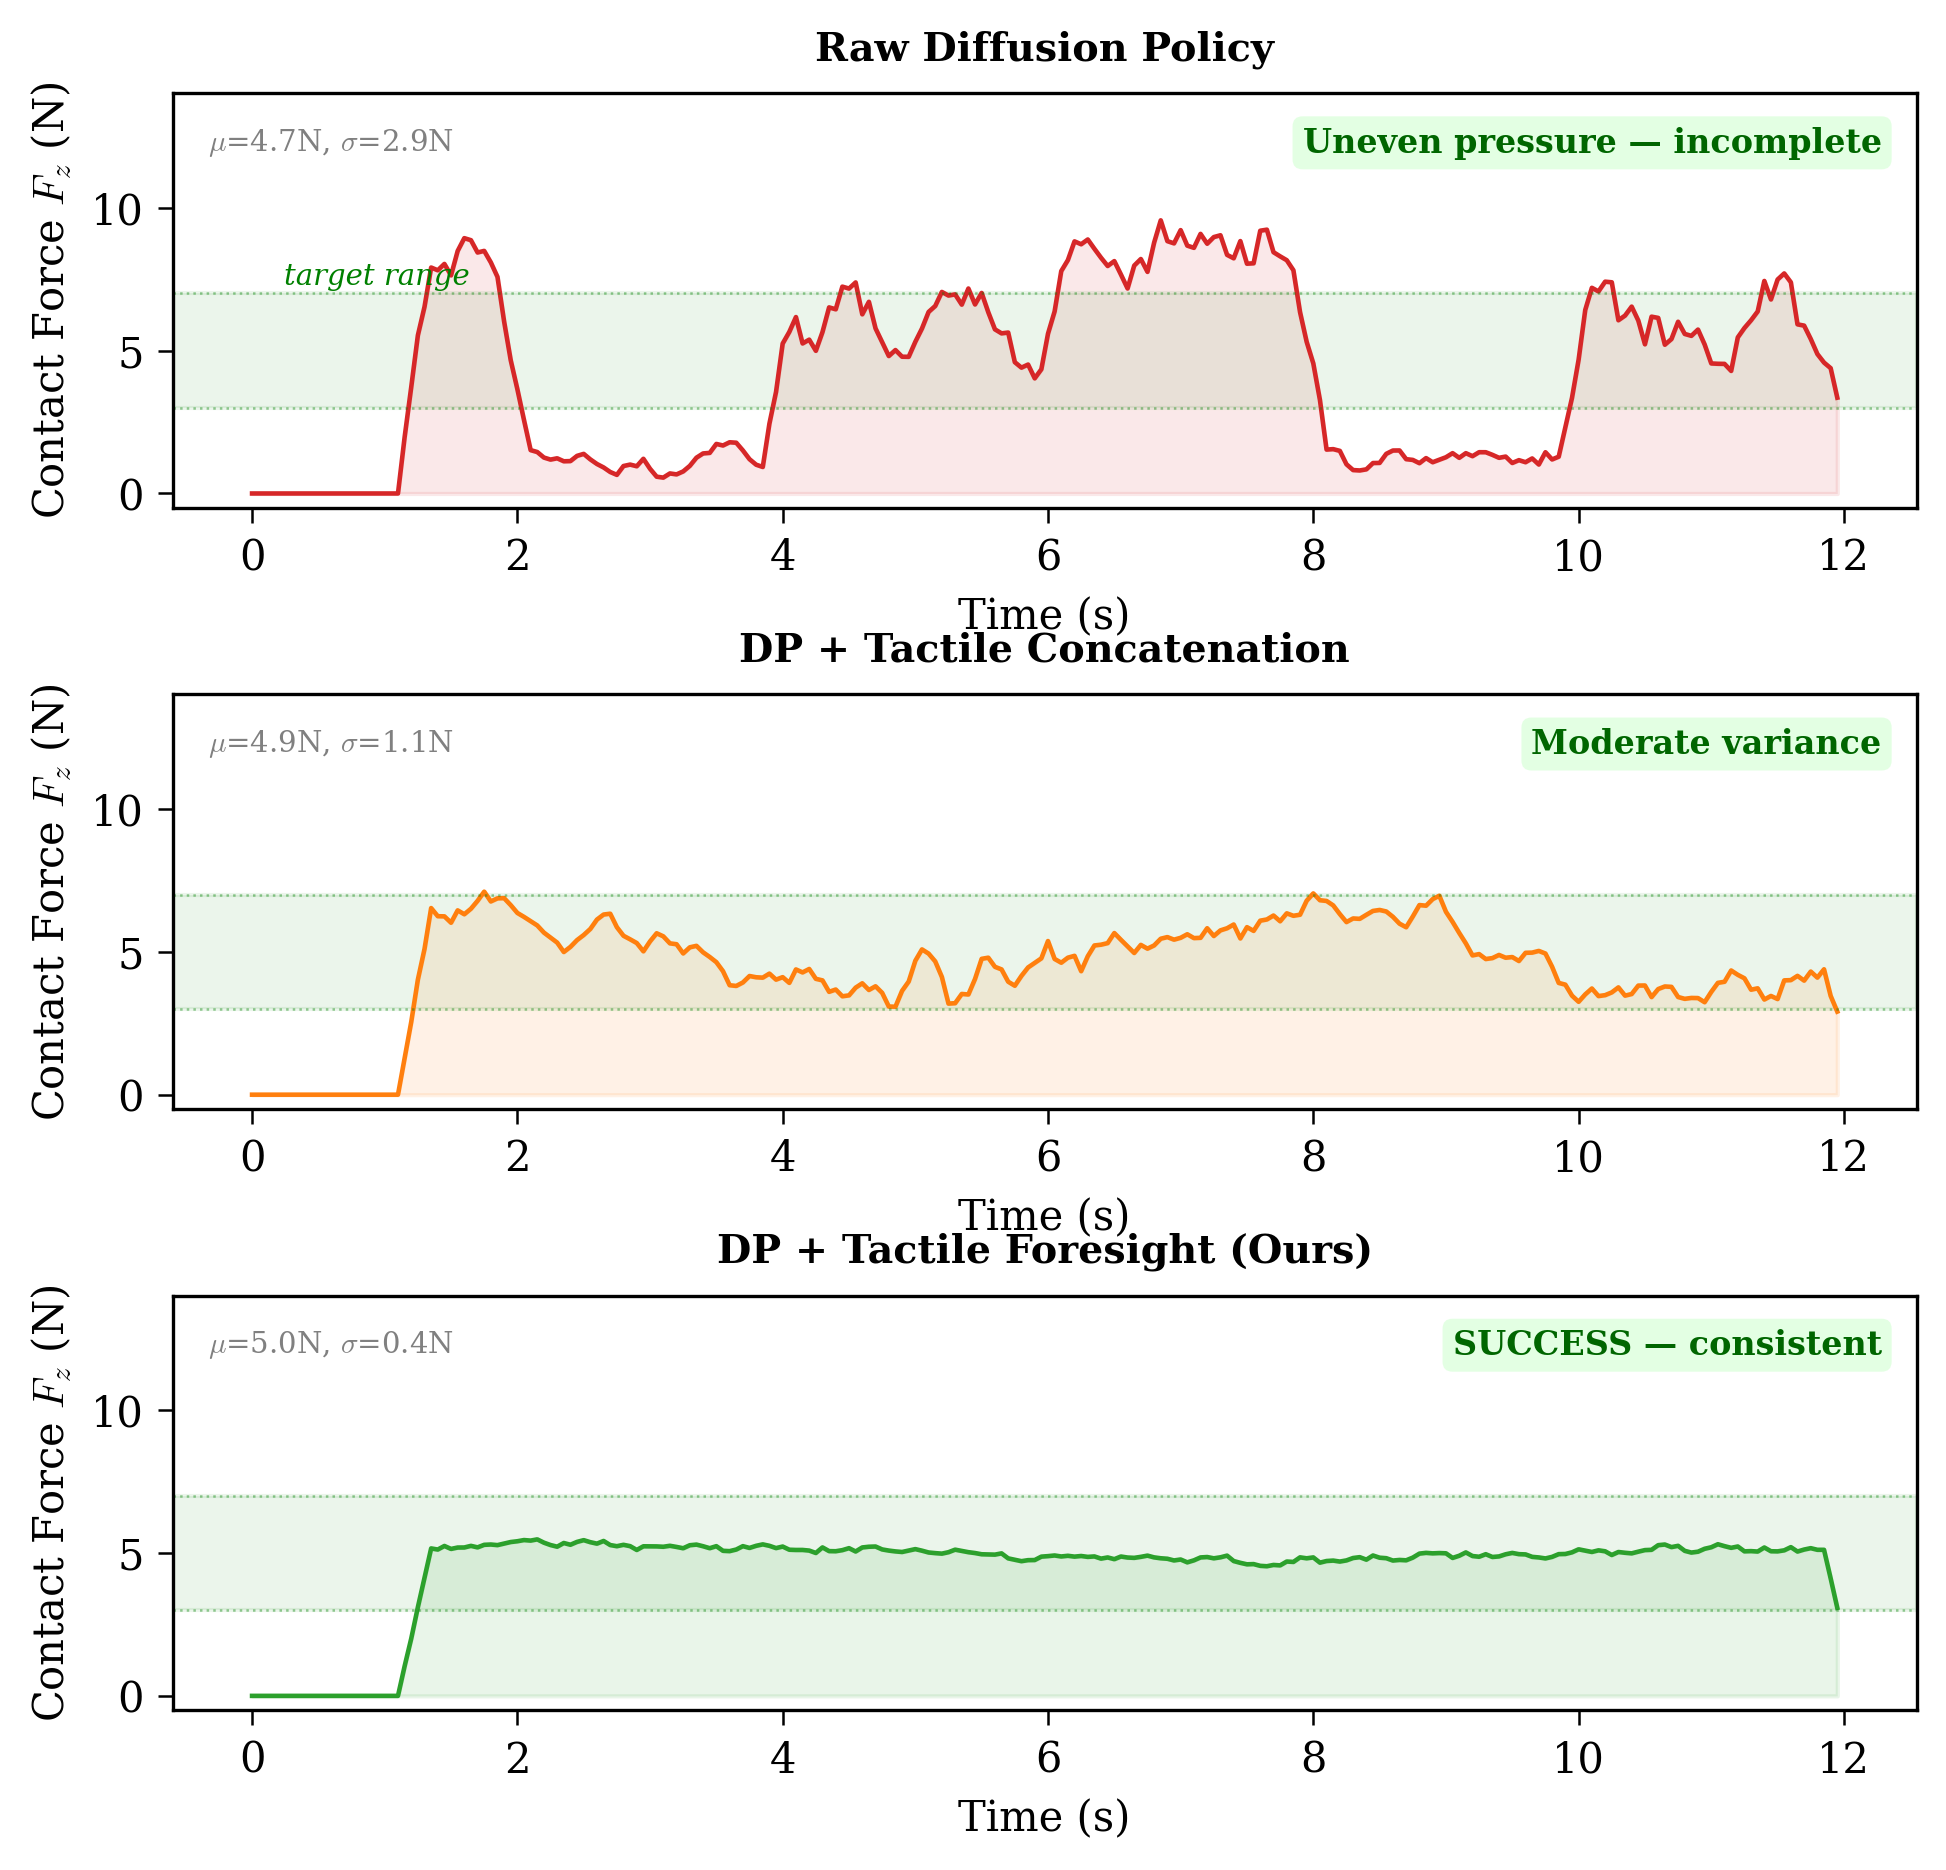
\includegraphics[width=0.92\textwidth]{force_board_wiping.png}
  \caption{Board wiping force traces. Raw DP produces unstable pressure and
  contact dropouts. Tactile concatenation improves the mean force but still
  exhibits moderate variation. \method{} keeps the force in the desired band
  with substantially lower variance.}
  \label{fig:appendix_force_board}
\end{figure*}

\begin{figure*}[t]
  \centering
  \includegraphics[width=0.92\textwidth]{force_vase_wiping.png}
  \caption{Vase wiping force traces. The curved fragile surface makes force
  stability more important than on a flat board. The guided policy maintains a
  lower-variance force profile and avoids the tip-over mode observed for raw
  DP.}
  \label{fig:appendix_force_vase}
\end{figure*}

\begin{figure*}[t]
  \centering
  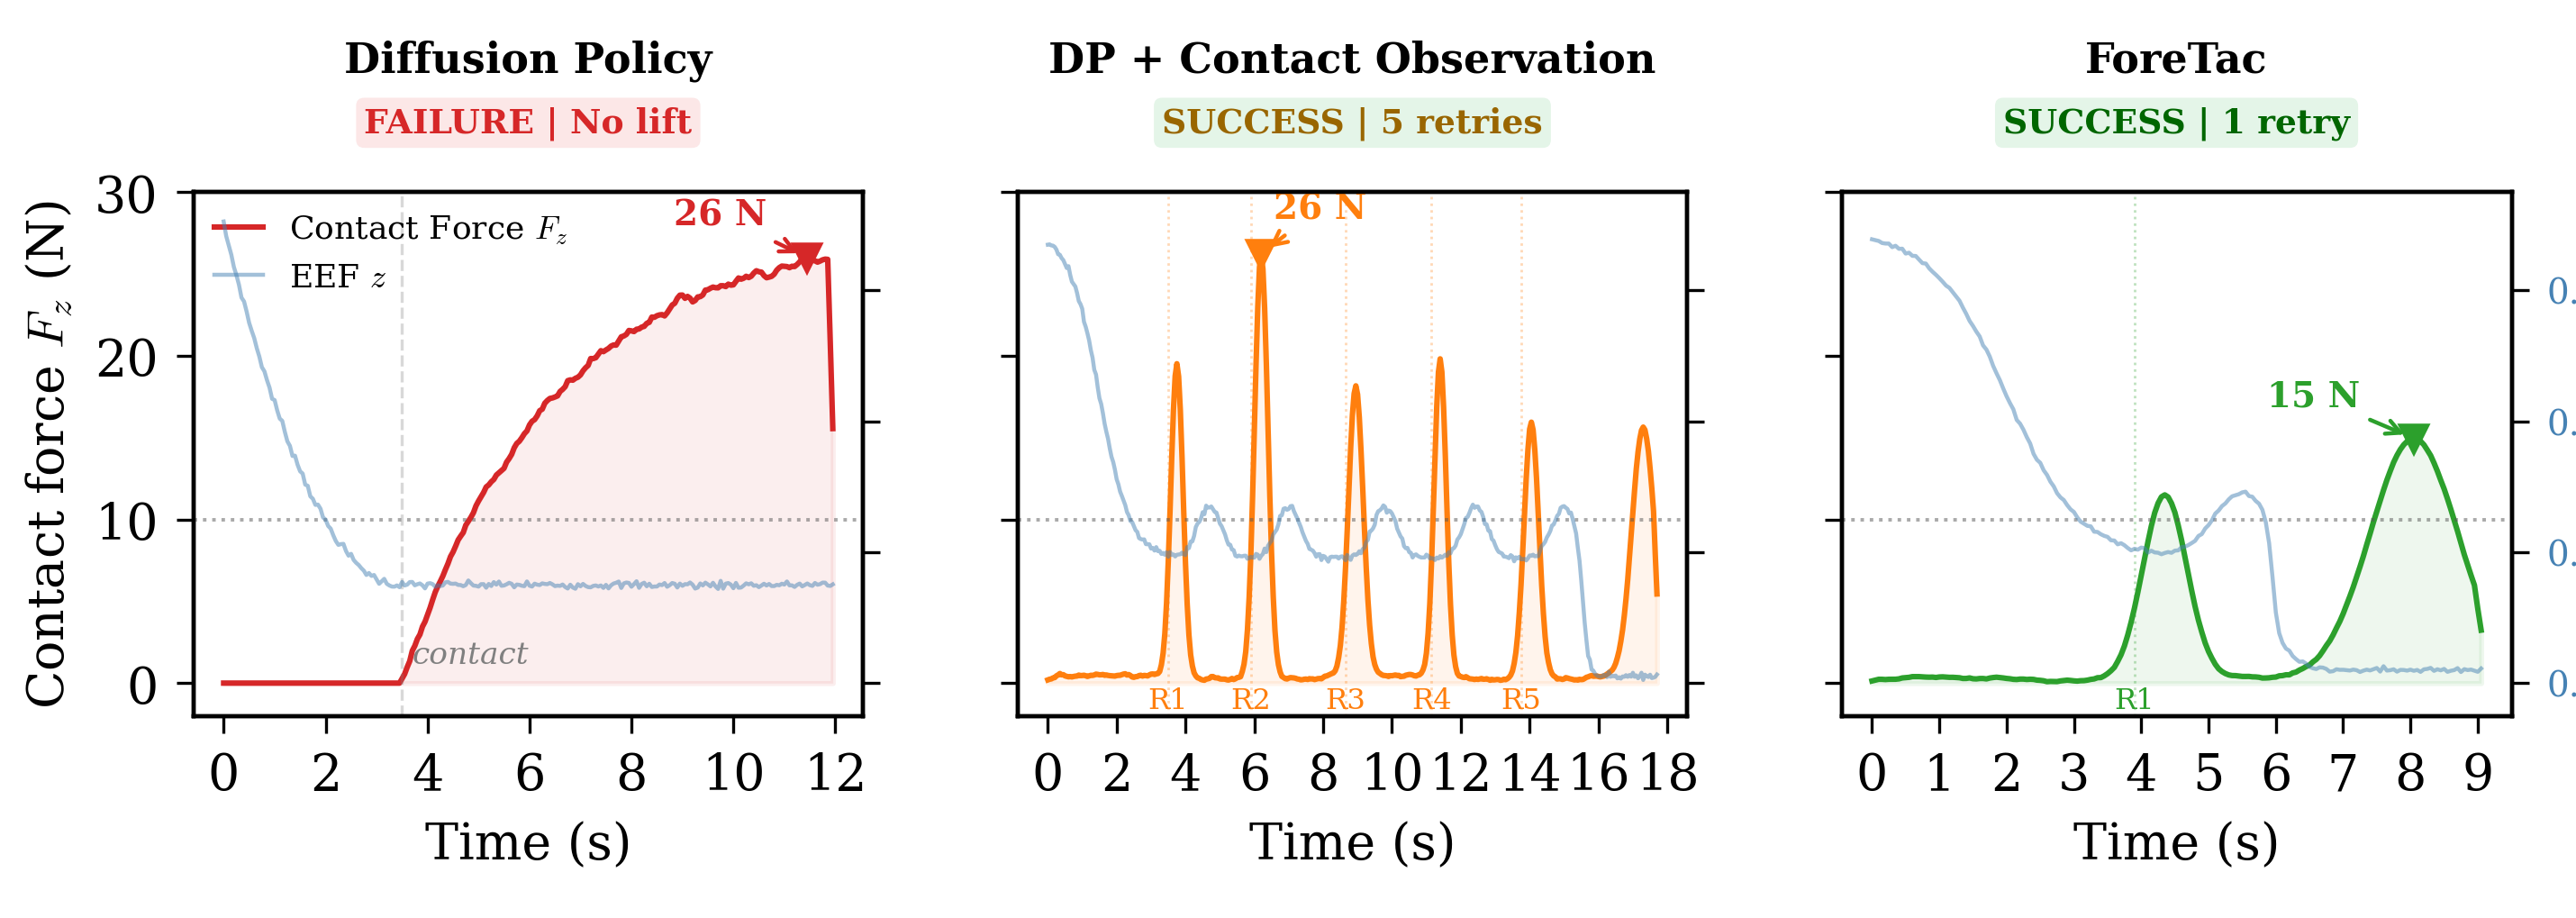
\includegraphics[width=0.92\textwidth]{force_real_3panel.png}
  \caption{Socket insertion force traces. Raw DP sustains high force and fails
  to lift after contact; tactile concatenation succeeds with repeated
  bounce-lift-reinsert cycles; \method{} reduces peak force and recovery time.}
  \label{fig:appendix_force_insertion}
\end{figure*}

\section{Main Comparison}
\label{sec:main_comparison}

Table~\ref{tab:main_comparison} is the current main rollout table. Each entry
reports success rate and successful trials over 20 attempts. Safe success is
the stricter subset that also satisfies the safety criteria defined in
Section~\ref{sec:data}.

\begin{table*}[t]
\caption{Main comparison across contact-rich manipulation tasks.}
\label{tab:main_comparison}
\centering
\setlength{\tabcolsep}{2.5pt}
\resizebox{\textwidth}{!}{%
\begin{tabular}{lcccccccccc}
\toprule
Method &
Board Succ. & Board Safe &
Vase Succ. & Vase Safe &
Vase Up-Down Succ. & Vase Up-Down Safe &
Card Succ. & Card Safe &
Chip Succ. & Chip Safe\\
\midrule
DP & 50\% (10/20) & 25\% (5/20) & 55\% (11/20) & 35\% (7/20) & 5\% (1/20) & 0\% (0/20) & 10\% (2/20) & 5\% (1/20) & 30\% (6/20) & 20\% (4/20)\\
DP+tactile & 60\% (12/20) & 50\% (10/20) & 60\% (12/20) & 50\% (10/20) & 40\% (8/20) & 30\% (6/20) & 35\% (7/20) & 30\% (6/20) & 40\% (8/20) & 35\% (7/20)\\
$\pi_{0.5}$ & 55\% (11/20) & 45\% (9/20) & 60\% (12/20) & 45\% (9/20) & 30\% (6/20) & 20\% (4/20) & 25\% (5/20) & 20\% (4/20) & 45\% (9/20) & 35\% (7/20)\\
RDP & 65\% (13/20) & 55\% (11/20) & 65\% (13/20) & 55\% (11/20) & 45\% (9/20) & 35\% (7/20) & 40\% (8/20) & 35\% (7/20) & 50\% (10/20) & 45\% (9/20)\\
\textbf{Ours} & \textbf{85\% (17/20)} & \textbf{80\% (16/20)} & \textbf{70\% (14/20)} & \textbf{65\% (13/20)} & \textbf{55\% (11/20)} & \textbf{50\% (10/20)} & \textbf{55\% (11/20)} & \textbf{50\% (10/20)} & \textbf{75\% (15/20)} & \textbf{70\% (14/20)}\\
\bottomrule
\end{tabular}%
}
\end{table*}

The main comparison separates two improvements. First, tactile concatenation
helps the base policy by adding current contact evidence, but it remains
reactive. Second, \method{} uses predicted tactile consequences before action
execution, giving the scorer a way to penalize contact dropout, excessive
force, and unstable contact earlier in the action chunk. The largest gains are
on tasks where visual geometry is insufficient to infer contact quality: board
wiping, chip grasping, and socket-style insertion.

\section{Ablation Study}
\label{sec:ablation}

Table~\ref{tab:ablation} isolates the role of tactile observations, foresight,
and guided denoising. DP Vision uses only visual/proprioceptive observations.
TacConcat adds current tactile latent features to the policy. Only Foresight
uses future tactile prediction without the full denoising guidance route.
DP Guide is the complete predict-score-guide system.

\begin{table*}[t]
\caption{Ablation study. Each entry reports success over 20 attempts and safe
success over the same 20 attempts.}
\label{tab:ablation}
\centering
\setlength{\tabcolsep}{2.5pt}
\resizebox{\textwidth}{!}{%
\begin{tabular}{lcccccccccc}
\toprule
Variant &
Board Succ. & Board Safe &
Vase Succ. & Vase Safe &
Vase Up-Down Succ. & Vase Up-Down Safe &
Card Succ. & Card Safe &
Chip Succ. & Chip Safe\\
\midrule
DP Vision & 50\% (10/20) & 35\% (7/20) & 55\% (11/20) & 35\% (7/20) & 10\% (2/20) & 5\% (1/20) & 10\% (2/20) & 5\% (1/20) & 30\% (6/20) & 20\% (4/20)\\
TacConcat & 60\% (12/20) & 50\% (10/20) & 60\% (12/20) & 50\% (10/20) & 40\% (8/20) & 30\% (6/20) & 35\% (7/20) & 30\% (6/20) & 40\% (8/20) & 35\% (7/20)\\
Only Foresight & 60\% (12/20) & 55\% (11/20) & 65\% (13/20) & 55\% (11/20) & 45\% (9/20) & 35\% (7/20) & 40\% (8/20) & 35\% (7/20) & 55\% (11/20) & 50\% (10/20)\\
\textbf{DP Guide} & \textbf{85\% (17/20)} & \textbf{80\% (16/20)} & \textbf{70\% (14/20)} & \textbf{65\% (13/20)} & \textbf{55\% (11/20)} & \textbf{50\% (10/20)} & \textbf{55\% (11/20)} & \textbf{50\% (10/20)} & \textbf{75\% (15/20)} & \textbf{70\% (14/20)}\\
\bottomrule
\end{tabular}%
}
\end{table*}

The ablation suggests that current tactile input is useful but insufficient:
TacConcat improves over vision-only DP, while Only Foresight improves safety on
several tasks by exposing future contact. The full DP Guide variant gives the
largest improvement because it uses foresight not only for representation, but
also as a differentiable contact-quality objective during late denoising.

\section{Insertion Benchmark}
\label{sec:insertion}

The socket insertion benchmark uses 20 trials per method. Besides success, the
task records retry count, maximum observed contact force, mean peak force, and
recovery time from peak force to below 2 N.

\begin{table}[t]
\caption{Peg-in-hole / socket insertion benchmark.}
\label{tab:insertion_appendix}
\centering
\resizebox{\columnwidth}{!}{%
\begin{tabular}{lccccc}
\toprule
Method & Succ. $\uparrow$ & Retry $\downarrow$ & Max F (N) $\downarrow$ & Peak F (N) $\downarrow$ & Recover (s) $\downarrow$\\
\midrule
Raw DP & 35\% (7/20) & 0 & 28.1 & 24.3 & --\\
DP+Tac & 60\% (12/20) & 4.2 & 26.4 & 21.5 & 1.85\\
DP+Foresight & 85\% (17/20) & 1.1 & 15.2 & 12.8 & 0.42\\
RDT+Foresight & \textbf{90\% (18/20)} & \textbf{0.9} & \textbf{14.1} & \textbf{11.5} & \textbf{0.35}\\
\bottomrule
\end{tabular}%
}
\end{table}

Raw DP has no explicit recovery behavior, so ``retry'' is reported as zero in
failed no-lift trials rather than as a sign of stable insertion. DP+Tac can
recover, but the recovery appears as repeated high-force contact cycles.
Foresight-guided variants reduce both the number of retries and the magnitude
of force peaks.

\section{Backbone Adaptation}
\label{sec:backbone}

\method{} is designed to wrap any chunk-based action generator. For DP, the
guidance gradient is applied directly to the denoising action sample. For RDP,
the same predicted-contact score is attached to the reactive diffusion
transformer action chunk. For $\pi_{0.5}$, the current adaptation keeps the VLA
backbone in a flow-matching action-generation role and appends tactile latent
tokens to the policy prefix; the foresight branch remains the action-conditioned
contact consequence model. In all cases, the contact-quality scorer is outside
the base policy and can be evaluated independently.

\begin{table}[t]
\caption{Backbone adaptation summary.}
\label{tab:backbone_adapt}
\centering
\resizebox{\columnwidth}{!}{%
\begin{tabular}{lll}
\toprule
Backbone & Adaptation & Additional policy training\\
\midrule
DP & late denoising action update & task DP checkpoint\\
RDP & same score on reactive action chunk & task RDP checkpoint\\
$\pi_{0.5}$ & tactile latent prefix + flow-matching action chunk & $\pi_{0.5}$ fine-tuning / adapter\\
ForeAR & autoregressive foresight baseline & \tbd{}\\
\bottomrule
\end{tabular}%
}
\end{table}

\section{Open Items for Final Appendix}
\label{sec:open_items}

The following items should be filled before camera-ready submission:
\begin{itemize}
\item Replace smoke preference-order accuracy with the full paired rollout
validation once all positive/negative pairs are collected.
\item Fill the chip grasping data inventory and add the missing chip force
curve if it is used in the final paper.
\item Add final $\pi_{0.5}$ and ForeAR rollout rows if they are part of the
main comparison.
\item Add qualitative panels for all five tasks using the final visual assets
from the project webpage.
\item Re-run the horizon table after the final action-conditioned foresight
checkpoint is selected, and keep the action-conditioned config archived with
the appendix source.
\end{itemize}

\end{document}
